\documentclass{article}

\usepackage{tikz}

\usepackage{gnuplot-lua-tikz}



\begin{document}

\begin{figure}

  \centering
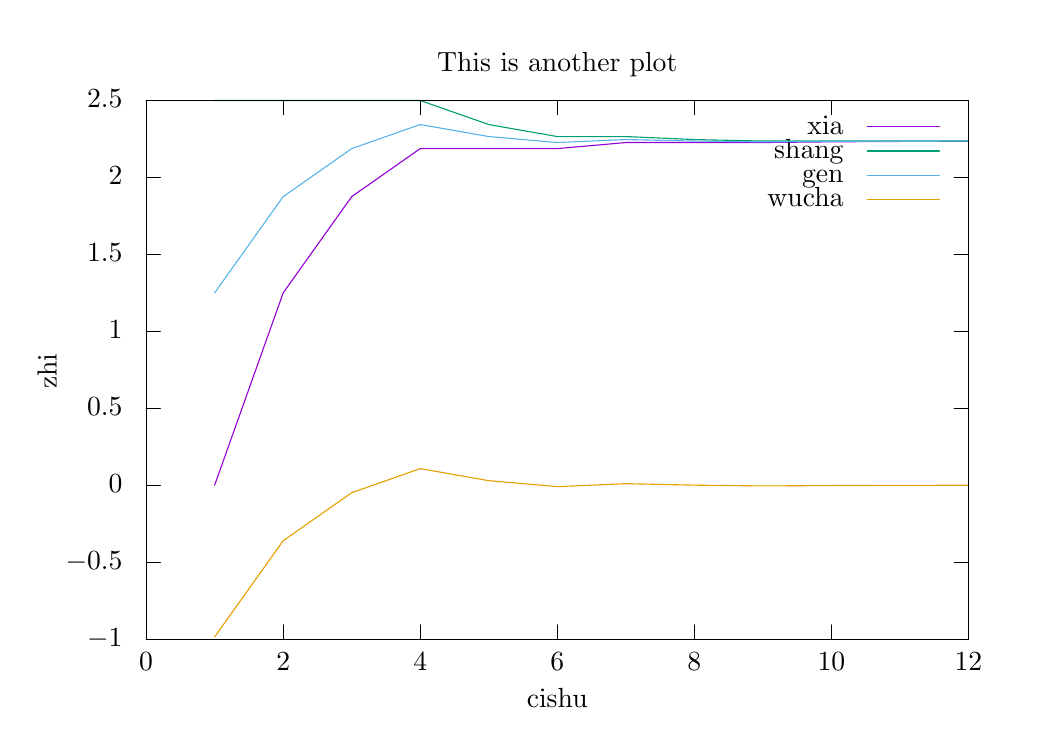
\begin{tikzpicture}[gnuplot]
%% generated with GNUPLOT 5.2p8 (Lua 5.3; terminal rev. Nov 2018, script rev. 108)
%% Mon 04 Jul 2022 01:59:49 PM CST
\path (0.000,0.000) rectangle (12.500,8.750);
\gpcolor{color=gp lt color border}
\gpsetlinetype{gp lt border}
\gpsetdashtype{gp dt solid}
\gpsetlinewidth{1.00}
\draw[gp path] (1.504,0.985)--(1.684,0.985);
\draw[gp path] (11.947,0.985)--(11.767,0.985);
\node[gp node right] at (1.320,0.985) {$-1$};
\draw[gp path] (1.504,1.962)--(1.684,1.962);
\draw[gp path] (11.947,1.962)--(11.767,1.962);
\node[gp node right] at (1.320,1.962) {$-0.5$};
\draw[gp path] (1.504,2.939)--(1.684,2.939);
\draw[gp path] (11.947,2.939)--(11.767,2.939);
\node[gp node right] at (1.320,2.939) {$0$};
\draw[gp path] (1.504,3.916)--(1.684,3.916);
\draw[gp path] (11.947,3.916)--(11.767,3.916);
\node[gp node right] at (1.320,3.916) {$0.5$};
\draw[gp path] (1.504,4.894)--(1.684,4.894);
\draw[gp path] (11.947,4.894)--(11.767,4.894);
\node[gp node right] at (1.320,4.894) {$1$};
\draw[gp path] (1.504,5.871)--(1.684,5.871);
\draw[gp path] (11.947,5.871)--(11.767,5.871);
\node[gp node right] at (1.320,5.871) {$1.5$};
\draw[gp path] (1.504,6.848)--(1.684,6.848);
\draw[gp path] (11.947,6.848)--(11.767,6.848);
\node[gp node right] at (1.320,6.848) {$2$};
\draw[gp path] (1.504,7.825)--(1.684,7.825);
\draw[gp path] (11.947,7.825)--(11.767,7.825);
\node[gp node right] at (1.320,7.825) {$2.5$};
\draw[gp path] (1.504,0.985)--(1.504,1.165);
\draw[gp path] (1.504,7.825)--(1.504,7.645);
\node[gp node center] at (1.504,0.677) {$0$};
\draw[gp path] (3.245,0.985)--(3.245,1.165);
\draw[gp path] (3.245,7.825)--(3.245,7.645);
\node[gp node center] at (3.245,0.677) {$2$};
\draw[gp path] (4.985,0.985)--(4.985,1.165);
\draw[gp path] (4.985,7.825)--(4.985,7.645);
\node[gp node center] at (4.985,0.677) {$4$};
\draw[gp path] (6.726,0.985)--(6.726,1.165);
\draw[gp path] (6.726,7.825)--(6.726,7.645);
\node[gp node center] at (6.726,0.677) {$6$};
\draw[gp path] (8.466,0.985)--(8.466,1.165);
\draw[gp path] (8.466,7.825)--(8.466,7.645);
\node[gp node center] at (8.466,0.677) {$8$};
\draw[gp path] (10.207,0.985)--(10.207,1.165);
\draw[gp path] (10.207,7.825)--(10.207,7.645);
\node[gp node center] at (10.207,0.677) {$10$};
\draw[gp path] (11.947,0.985)--(11.947,1.165);
\draw[gp path] (11.947,7.825)--(11.947,7.645);
\node[gp node center] at (11.947,0.677) {$12$};
\draw[gp path] (1.504,7.825)--(1.504,0.985)--(11.947,0.985)--(11.947,7.825)--cycle;
\node[gp node center,rotate=-270] at (0.292,4.405) {zhi};
\node[gp node center] at (6.725,0.215) {cishu};
\node[gp node center] at (6.725,8.287) {This is another plot};
\node[gp node right] at (10.479,7.491) {xia};
\gpcolor{rgb color={0.580,0.000,0.827}}
\draw[gp path] (10.663,7.491)--(11.579,7.491);
\draw[gp path] (2.374,2.939)--(3.245,5.382)--(4.115,6.604)--(4.985,7.214)--(5.855,7.214)%
  --(6.726,7.214)--(7.596,7.291)--(8.466,7.291)--(9.336,7.291)--(10.207,7.300)--(11.077,7.305)%
  --(11.947,7.307);
\gpcolor{color=gp lt color border}
\node[gp node right] at (10.479,7.183) {shang};
\gpcolor{rgb color={0.000,0.620,0.451}}
\draw[gp path] (10.663,7.183)--(11.579,7.183);
\draw[gp path] (2.374,7.825)--(3.245,7.825)--(4.115,7.825)--(4.985,7.825)--(5.855,7.520)%
  --(6.726,7.367)--(7.596,7.367)--(8.466,7.329)--(9.336,7.310)--(10.207,7.310)--(11.077,7.310)%
  --(11.947,7.310);
\gpcolor{color=gp lt color border}
\node[gp node right] at (10.479,6.875) {gen};
\gpcolor{rgb color={0.337,0.706,0.914}}
\draw[gp path] (10.663,6.875)--(11.579,6.875);
\draw[gp path] (2.374,5.382)--(3.245,6.604)--(4.115,7.214)--(4.985,7.520)--(5.855,7.367)%
  --(6.726,7.291)--(7.596,7.329)--(8.466,7.310)--(9.336,7.300)--(10.207,7.305)--(11.077,7.307)%
  --(11.947,7.309);
\gpcolor{color=gp lt color border}
\node[gp node right] at (10.479,6.567) {wucha};
\gpcolor{rgb color={0.902,0.624,0.000}}
\draw[gp path] (10.663,6.567)--(11.579,6.567);
\draw[gp path] (2.374,1.012)--(3.245,2.234)--(4.115,2.844)--(4.985,3.150)--(5.855,2.997)%
  --(6.726,2.921)--(7.596,2.959)--(8.466,2.940)--(9.336,2.930)--(10.207,2.935)--(11.077,2.937)%
  --(11.947,2.939);
\gpcolor{color=gp lt color border}
\draw[gp path] (1.504,7.825)--(1.504,0.985)--(11.947,0.985)--(11.947,7.825)--cycle;
%% coordinates of the plot area
\gpdefrectangularnode{gp plot 1}{\pgfpoint{1.504cm}{0.985cm}}{\pgfpoint{11.947cm}{7.825cm}}
\end{tikzpicture}
\end{figure}

\end{document}
